\documentclass[12pt,a4paper]{article}

\usepackage{fontspec}
\IfFontExistsTF{Times New Roman}
  {\setmainfont{Times New Roman}}
  {\IfFontExistsTF{CMU Serif}
    {\setmainfont{CMU Serif}}
    {\setmainfont{DejaVu Serif}}}
\IfFontExistsTF{Cascadia Mono}
  {\setmonofont{Cascadia Mono}}
  {\IfFontExistsTF{DejaVu Sans Mono}
    {\setmonofont{DejaVu Sans Mono}}
    {\setmonofont{CMU Typewriter Text}}}
\usepackage{geometry}
\geometry{left=25mm,right=15mm,top=20mm,bottom=20mm}
\setlength{\emergencystretch}{3em}
\usepackage{amsmath}
\usepackage{fvextra}
\usepackage{graphicx}
\usepackage{hyperref}
\hypersetup{hidelinks}

\title{Отчёт по задаче <<Города и дороги>>}
\author{Смола Артём, группа 23.Б08}
\date{}

\begin{document}
\maketitle

\section{Постановка задачи}
Дан связный неориентированный граф: города --- вершины, дороги --- рёбра с весами (длинами).
Заданы $k$ столиц, каждая столица соответствует отдельному государству.
Требуется распределить все города между государствами по правилам:
\begin{enumerate}
    \item Изначально в каждом государстве находится только его столица.
    \item Далее государства ходят по очереди от 1 до $k$.
    \item На ходе государство присоединяет один ближайший незанятый город, который имеет дорогу хотя бы к одному уже принадлежащему ему городу.
\end{enumerate}
Нужно вывести для каждого государства список принадлежащих ему городов в порядке присоединения.

\section{Принцип решения}
Для каждого государства используется отдельная приоритетная очередь.
Её элемент содержит:
\begin{itemize}
    \item длину дороги;
    \item номер кандидата-города;
    \item город данного государства, из которого найден кандидат.
\end{itemize}

Алгоритм:
\begin{enumerate}
    \item Считать граф списками смежности.
    \item Пометить столицы как уже занятые соответствующими государствами.
    \item Для каждой столицы добавить в её очередь все исходящие рёбра к незанятым городам.
    \item Пока есть незанятые города, циклически пройти по государствам:
    \begin{enumerate}
        \item удалить из вершины очереди устаревшие записи (если город уже занял кто-то другой);
        \item взять минимального кандидата;
        \item присоединить город к текущему государству;
        \item добавить в очередь рёбра из нового города к ещё незанятым городам.
    \end{enumerate}
\end{enumerate}

Алгоритм полностью реализует правило поочерёдного присоединения ближайшего доступного города.
При равенстве длины в очереди применяется правило разрешения равенств:
сначала по меньшему номеру города, затем по меньшему номеру города-источника.

\section{Корректность}
Инвариант: после каждого присоединения у каждого государства его множество городов
остается связным, поскольку новый город всегда присоединяется по ребру к уже принадлежащему городу.
Цикл ходов строго следует правилу задачи: государства ходят по порядку от $1$ до $k$.
На каждом ходе выбирается минимальный допустимый кандидат из очереди текущего государства.
Следовательно, порядок присоединений в программе совпадает с постановкой задачи.

\section{Ограничения реализации}
\begin{itemize}
    \item входной граф должен быть связным;
    \item при несвязном графе программа завершает работу с ошибкой;
    \item длины дорог предполагаются неотрицательными.
\end{itemize}

\section{Исходный код}
Исходный код программы и тестовые данные доступны в репозитории GitHub:
\url{https://github.com/artem-smola/formal_lang}.

\section{Код программы}

Код программы:

{\small
\VerbatimInput[
    fontsize=\footnotesize,
    breaklines=true,
    breakanywhere=true
]{../../Code/main.cpp}
}

\section{Демонстрация работы программы}
\subsection*{1) Входные данные}
\textbf{Рассматриваемый тест:} \texttt{test1}.

Формат входных данных:
\begin{enumerate}
    \item $n,\,m$ --- число городов и число дорог.
    \item Далее $m$ строк вида $i\ j\ len$, где $i$ и $j$ --- номера городов, $len$ --- длина дороги.
    \item $k$ --- число государств (число столиц).
    \item Далее $k$ чисел --- номера столиц.
\end{enumerate}
Ограничения: граф связный, нумерация городов --- от $1$ до $n$.

{\small
\VerbatimInput[
    fontsize=\footnotesize,
    breaklines=true,
    breakanywhere=true
]{../../Code/tests/test1.in}
}

\subsection*{2) Вывод}

\begin{center}
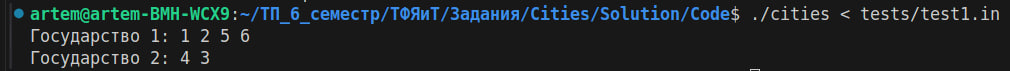
\includegraphics[
    width=\textwidth,
    keepaspectratio
]{assets/terminal_output_test1.png}
\end{center}

\subsection*{3) Визуализация}
\IfFileExists{../../Visualization/test1.png}{
\begin{center}

\includegraphics[
    width=\textwidth,
    height=0.38\textheight,
    keepaspectratio
]{../../Visualization/test1.png}
\end{center}
}{
\textbf{Файл визуализации:} \texttt{../../Visualization/test1.dot}

{\small
\VerbatimInput[
    fontsize=\footnotesize,
    breaklines=true,
    breakanywhere=true
]{../../Visualization/test1.dot}
}
}

\subsection*{4) Описание результата}

По результату для данного теста:
\begin{itemize}
    \item государство 1 получает города $\{1, 2, 5, 6\}$;
    \item государство 2 получает города $\{4, 3\}$.
\end{itemize}
Это соответствует пошаговому присоединению ближайших доступных городов при чередовании ходов государств.

\subsection*{5) Дополнительный граничный тест}
Для \texttt{test3} проверяется ситуация с близкими длинами рёбер и выбором по правилу разрешения равенств:

\textbf{Входные данные теста \texttt{test3}:}

{\small
\VerbatimInput[
    fontsize=\footnotesize,
    breaklines=true,
    breakanywhere=true
]{../../Code/tests/test3.in}
}

\[
\text{Государство 1: }1,\,2,\,4,\quad
\text{Государство 2: }5,\,3.
\]
Это демонстрирует детерминированность выбора при равных/близких кандидатах.

\section{Анализ сложности}
Обозначения: $n$ --- число городов, $m$ --- число дорог, $k$ --- число государств.

Построение списков смежности: $O(m)$.

Каждое ребро может быть добавлено в очереди ограниченное число раз (по мере роста состояний), а каждая операция с очередью стоит $O(\log S)$, где $S$ --- текущий размер очереди. В сумме время работы:
\[
O(m \log m)
\]
для типичного и худшего случая данной реализации.

Память:
\[
O(n + m)
\]
на граф, массивы принадлежности городов и структуры очередей.

\end{document}
